% Template for SE Project software documentation
% (c) Farhad Mehta 2021
% !TEX program = xelatex

\documentclass[11pt, oneside, a4paper]{book}

% File containing the commands and definitions
% that are used throughout this project.

% Set input encoding
\usepackage[utf8]{inputenc}

% For creating coloured text and backgrounds
\usepackage[table,xcdraw]{xcolor}

% For creating compact lists
\usepackage{paralist}

% To get the current date and time
\usepackage{datetime2}

% For including graphics
\usepackage{graphicx}

% For landscape pages
\usepackage{lscape}

% For tables longer than one page (includes page breaks)
\usepackage{longtable}

% Custom commands

\newcommand{\todo}[1]{TODO: {#1}}

% The following command indicates that its content consists of instructions
% Even if it does not do anything, it is still a good idea to keep instructions within the `instruction` tag to separate them from the rest of the text. One could then typeset them differently, or choose to remove them form the document by redefining the command definition 
\newcommand{\instructions}[1]{#1}

% Uncomment the following command to remove all instructions
% \newcommand{\instructions}[1]{}

% Uncomment the following to make instructions appear in coloured boxes
% Note: The changes within `\instruction` are not visible in latexdiff when they are typeset in this way
% \usepackage{tcolorbox}
% \newcommand{\instructions}[1]{
%     \begin{tcolorbox}[sharp corners, colback=green!30, colframe=green!80!blue, title=Instructions]
%         #1
%     \end{tcolorbox}
% }

% Uncomment the following to make instructions appear in colour.
% Note: The changes within `\instructions` are not visible in latexdiff when they are typeset in this way
% \newcommand{\instructions}[1]{ { \color{blue} #1 } }

% Get a git version description roughly using the idea in  
% https://blog.wxm.be/2013/08/20/automated-git-commit-number-in-latex.html
% Note that the file that is included needs to be generated before the document is built.
% Refer to the makefile for further details.
\IfFileExists{../gitDescription.tmp}
{\newcommand{\gitDescription}{\input{../gitDescription.tmp}}}
{\newcommand{\gitDescription}{Not available}}

% Note: Importing hyperref must be done towards the end since it
% redefines many macros
%
% Note:
%  The following packages must be imported *before* hyperref:
%  
%  The following packages must be imported *after* hyperref:
%    amsrefs, geometry
\usepackage{hyperref}

%\usepackage{geometry}
\usepackage[a4paper, left=3cm, right=3cm, top=2cm]{geometry}

\usepackage{listings}

\usepackage{textcomp}

% options for package geometry (influences writable area on page)
% \geometry{a4paper, top=2cm, bottom=2cm}

\usepackage{float}


\hypersetup{
    pdfauthor={Benjamin Plattner, Jan Untersander, Olivier Lischer, Pascal Lehmann, Petra Heeb},
    pdftitle={SE Project KubeWatch documentation},
}

\begin{document}

\pagestyle{empty}

\frontmatter

\begin{titlepage}

    \begin{center}

        \fbox{\Huge KubeWatch Documentation}

        \vspace{1 cm}

        {\Large SE Project \\ Documentation} \\

        \vspace{0.5cm}

        {\Huge KubeWatch}

        \vspace{0.5cm}

        Semester: Spring 2022

        \vspace{0.5 cm}

        % TODO: Create a logo that is less ugly
        
\includegraphics[height=4cm]{resources/se-project-logo.png}

        \vspace{0.5 cm}

        Version: 2.0 \\
        Date: \DTMnow \\
        Git Version: \gitDescription
        \vspace{1 cm}

        \begin{tabular}{rl}
            \textbf{Project Team:}    & Benjamin Plattner \\
                                      & Jan Untersander \\
                                      & Olivier Lischer \\
                                      & Pascal Lehmann \\
                                      & Petra Heeb \\
                                      &                    \\
            \textbf{Project Advisor:} & Laurent Metzger
        \end{tabular}

        \vspace{0.5cm}

        
\includegraphics[height=2cm]{resources/ost-logo.png}\\

        \vspace{0.5cm}
        School of Computer Science\\
        OST Eastern Switzerland University of Applied Sciences

    \end{center}

\end{titlepage}

\tableofcontents
% \chapter*{Instructions for using this template}

\instructions{
    \begin{enumerate}
        \item The main aim of this document template is to allow you to start working on your project documentation as quickly as possible.
        \item In addition to recommending a rough structure for your project documentation, this template also contains instructions related to the content and execution your project. Instructional text is typeset within the \LaTeX\ \texttt{instructions} command defined in \texttt{custom.tex}. Make sure that your final submission does not contain any instructional texts.
        \item The basic defaults that \LaTeX\ provides have been used whenever possible in order to keep the template as simple as possible for beginners. One can do better. \LaTeX\ also provides additional features such as glossaries, abbreviation lists and indexes that you may find useful. Feel free to customise the typesetting and content of this document as per your requirements, tastes and wishes as you progress with the project.
        \item Here is an example of a bibliography reference: \cite{larman_applyingUmlAndPatterns_2004}
    \end{enumerate}
}



\mainmatter

% \part{Management Summary}
% \chapter*{Management Summary}

\instructions{
    Even though this is the first chapter of your document, it is typically the last one filled with content. The \textit{Management Summary} is a \textbf{brief and high-level summary} of your project. It should give any reader unfamiliar to the project an overview of the contents included later in the document.
    
    \bigskip
    
    A common structure is:
    
    \begin{itemize}
        \item What is the problem we wanted to solve?
        \item How did we solve the problem?
        \item Does your solution solve the problem in a successful way?
        \item Will there be consecutive projects based on your work?
    \end{itemize}
    
    Diagrams and images work very well in this chapter, especially screenshots of your software.
    
    \bigskip
    
    One final remark: a well written management summary is a good starting point for your \textbf{Project Presentation}, as you will address a similar audience there.
}



\part{Product Documentation}
\chapter{Vision}

% \instructions{
%     Describe the vision for the product on 1 page as covered in the SEP1 module.
% }

%\paragraph{KubeWatch} is a monitoring application for Kubernetes (K8S), intended for technical users.
%It keeps track of multiple K8S nodes, records performance data over time and generates visualizations from the aggregated data.
%It can detect when a node goes down, which triggers a notification to the person in charge.
%We chose this topic because it combines multiple technical aspects, so that each team member can get something out of it.

\textbf{KubeWatch} is a monitoring web application to monitor Kubernetes clusters. This application is designed for technical users and requires some basic knowledge about kubernetes. With KubeWatch you can visualize and summarize various metrics of a cluster or individual nodes and different kubernetes workloads. With an adaptive interface, each user can view the metrics and visualizations according to their own preferences. In addition to visualization, KubeWatch has an alert function, for which thresholds on different metrics can be set in the web application by individual users. KubeWatch will use these metrics to calculate whether an alert needs to be sent or whether the value is still within the desired range. The are shown/sent via simple pop up notifications, email or other messaging applications. With this feature set, KubeWatch allows for easy monitoring and user-defined alerting.
\chapter{Requirements}

\section{Functional Requirements}
The functional requirements are written as a description in the GitLab issue\footnote{\url{https://gitlab.ost.ch/SEProj/2022-FS/g03-kubewatch/kubewatch/-/issues/55}}.

We do use Scrum.
Therefore, all estimates and other refinements are made every two weeks in the sprint meeting.

The User Stories are prioritised.
The higher a User Story is in the Story Board\footnote{\url{https://gitlab.ost.ch/SEProj/2022-FS/g03-kubewatch/kubewatch/-/boards/935}} the higher is the priority.


\section{Non-Functional Requirements}
The process for validating Non-Functional Requirements (NFRs) is to use automation tools wherever possible. We are currently setting up SonarQube and we will add as many of the defined metrics as possible. Those NFRs which we deem critical, but cannot be tracked by SonarQube will be validated at least once every sprint and confirmed by the validator during a regular sprint meeting.

\begin{table}[h!]
    \centering
      \caption{\label{tab:nfr-review}NFR reviews and changelog}
      \begin{tabular}{ | l | l | }
        \hline
        \textbf{Date} & \textbf{Changes} \\
        \hline
        15.03.22 & Created initial set of NFRs. \\
        \hline
        30.03.22 & Added NFR 5-10, Updated NFR-1 \\
        \hline
        01.04.22 & Updated NFR 5,7,8 \\
        \hline
      \end{tabular}
    \end{table}

\begin{center}
\begin{tabular}{ | m{8em} | m{25em}| } 
 \hline
 \textbf{ID} & NFR-1\\ 
 \hline
 \textbf{Requirement} & The software must have a good quality. \\
 \hline
 \textbf{Priority} & High\\
 \hline
 \textbf{Measure(s)} & The test coverage must be minimal 75\%.\\
 \hline
 \textbf{Process} & Use \textit{SonarQube} Coverage metrics. \\
 \hline
\end{tabular}
\end{center}

\begin{center}
\begin{tabular}{ | m{8em} | m{25em}| } 
 \hline
 \textbf{ID} & NFR-2\\ 
 \hline
 \textbf{Requirement} & The web interface must load fast.\\
 \hline
 \textbf{Priority} & High\\
 \hline
 \textbf{Measure(s)} & The response time must be under 5s.\\
 \hline
 \textbf{Process} & Use Browsers Developer Tools to verify the loading time.\\
 \hline
\end{tabular}
\end{center}

\begin{center}
\begin{tabular}{ | m{8em} | m{25em}| } 
 \hline
 \textbf{ID} & NFR-3\\ 
 \hline
 \textbf{Requirement} & The application memory usage must be minimal.\\
 \hline
 \textbf{Priority} & Medium\\
 \hline
 \textbf{Measure(s)} & The maximal memory usage must be less than 200 MB.\\
 \hline
 \textbf{Process} & Monitor the system over a given period of time.\\
 \hline
\end{tabular}
\end{center}

\begin{center}
\begin{tabular}{ | m{8em} | m{25em}| } 
 \hline
 \textbf{ID} & NFR-4\\ 
 \hline
 \textbf{Requirement} & The product must be implemented using Node.js and Kubernetes.\\
 \hline
 \textbf{Priority} & Low\\
 \hline
 \textbf{Measure(s)} & Only JS / TS files are used.\\
 \hline
 \textbf{Process} & Check the source code and the deployment infrastructure.\\
 \hline
\end{tabular}
\end{center}

\begin{center}
\begin{tabular}{ | m{8em} | m{25em}| } 
 \hline
 \textbf{ID} & NFR-5\\ 
 \hline
 \textbf{Requirement} & The product must be scalable for high availability.\\
 \hline
 \textbf{Priority} & Middle\\
 \hline
 \textbf{Measure(s)} & Software must run in a container environment.\\
 \hline
 \textbf{Process} & Let the software run in a container.\\
 \hline
\end{tabular}
\end{center}

\begin{center}
\begin{tabular}{ | m{8em} | m{25em}| } 
 \hline
 \textbf{ID} & NFR-6\\ 
 \hline
 \textbf{Requirement} & The Software must usable for a technical user.\\
 \hline
 \textbf{Priority} & High \\
 \hline
 \textbf{Measure(s)} & Technical User gives positive feedback.\\
 \hline
 \textbf{Process} & Have a technical user work with the software.\\
 \hline
\end{tabular}
\end{center}

\begin{center}
\begin{tabular}{ | m{8em} | m{25em}| } 
 \hline
 \textbf{ID} & NFR-7\\ 
 \hline
 \textbf{Requirement} & The software must handle absence of APIs it depends on.\\
 \hline
 \textbf{Priority} & High \\
 \hline
 \textbf{Measure(s)} & Software sends Notification about missing APIs.\\
 \hline
 \textbf{Process} & Let the software run without connection to any API.\\
 \hline
\end{tabular}
\end{center}

\begin{center}
\begin{tabular}{ | m{8em} | m{25em}| } 
 \hline
 \textbf{ID} & NFR-8\\ 
 \hline
 \textbf{Requirement} & The software must reconnect to APIs it depends on automatically.\\
 \hline
 \textbf{Priority} & Middle \\
 \hline
 \textbf{Measure(s)} & The software sends Notification that it is fully functional again.\\
 \hline
 \textbf{Process} & Start software without connection to any API and start APIs after software.\\
 \hline
\end{tabular}
\end{center}

\begin{center}
\begin{tabular}{ | m{8em} | m{25em}| } 
 \hline
 \textbf{ID} & NFR-9\\ 
 \hline
 \textbf{Requirement} & The software must be secure. \\
 \hline
 \textbf{Priority} & Middle \\
 \hline
 \textbf{Measure(s)} & The Security Rating must be at least a B. \\
 \hline
 \textbf{Process} & Use \textit{SonarQube} Security Rating metrics. \\
 \hline
\end{tabular}
\end{center}

\begin{center}
\begin{tabular}{ | m{8em} | m{25em}| } 
 \hline
 \textbf{ID} & NFR-10\\ 
 \hline
 \textbf{Requirement} & Code must be maintainable. \\
 \hline
 \textbf{Priority} & High \\
 \hline
 \textbf{Measure(s)} & The Maintainability Rating must be at least a B.\\
 \hline
 \textbf{Process} & Use \textit{SonarQube} Maintainability Rating metrics. \\
 \hline
\end{tabular}
\end{center}

% \chapter{Domain Analysis}

% \instructions{
%     Describe the problem domain using a domain model as covered in the SEP1 module.
% }

For KubeWatch's domain analysis we use a domain model to describe the project. It contains all necessary information to be self-explanatory.

\section{Domain Model}
The different elements in our domain model (see figure \ref{fig:domain-model}) are aligned with our functional requirements, which are specified in our repository. If there are any further enhancements planned which are outside the current scope, we will adjust and enhance the domain model accordingly.

\vspace{1cm}

\begin{figure}[h]
    \centering
    \caption{KubeWatch Domain Model}
    \label{fig:domain-model}
    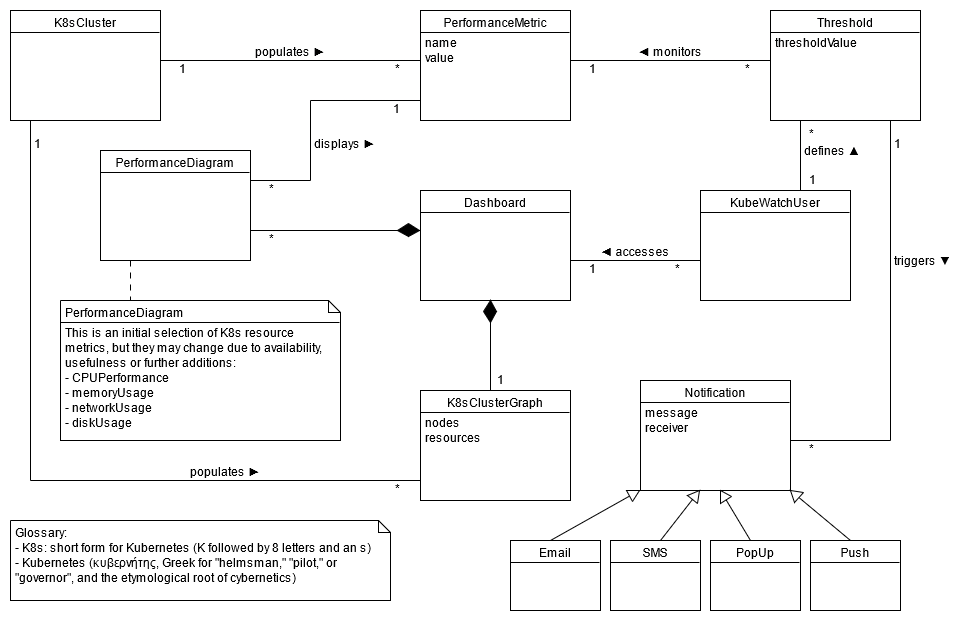
\includegraphics[width=\textwidth]{resources/domain_model.png}
\end{figure}
% \chapter{Architecture}

\instructions{
    Describe the architecture of your software as covered in the SEP2 module. The main goal of this chapter is describing the \textbf{technical implementation} in a way that a new team member can start working on the product as fast as possible.
    
    \begin{itemize}
        \item Use an existing template as a starting point (\texttt{arc42}, \texttt{C4 model}, ...)
        \item Focus on stable, high-level concepts rather than details
        \item Cover different views (static, dynamic, deployment, ...)
        \item Prefer diagrams over text (ideally UML)
        \item Explain the reasons behind your actions: \textit{Why did we build it like this?}
    \end{itemize}   
}
% \chapter{Quality Measures}

%% \instructions{
%%     Describe the quality measures applied in your project as covered in the SEP2 module. Things that might be included in this chapter:
    
%%     \begin{itemize}
%%         \item Organizational means like \textit{Merge Requests}, \textit{Definition of Done}, etc.
%%         \item Tools used to assess the quality of your product (linter, metrics, ...)
%%         \item Tools used to build and deploy your product (CI/CD)
%%         \item The \textit{Test Concept} used for testing your product
%%     \end{itemize}
    
%%     Try to avoid duplication with other chapters such as the \textit{Project Plan}. Work with cross-references when appropriate.
%% }

\section{Definition of Ready / Definition of Done}

\subsection{DoR}

\subsection{DoD}
The following \textit{Definition of Done} was taken and adjusted to our needs from scrum-events.de \cite{scrumEvents_wasIstDieDod}.
\begin{itemize}
  \item The code is finished and versioned by git
  \item The code was review or developed using pair programming
  \item The code fulfills the coding guidelines in \ref{guidelines-web-api}
  \item The code has unit tests (where possible) and these are green
  \item The documentation was updated
  \item No critical bugs are known
\end{itemize}


\section{Apply Quality standard}
To provide a certain code standard and quality some coding guidelines were specified.
These guidelines can be found in the section \ref{guidelines-web-api}.
For the Kubernetes similar guidelines were specified.
You can find them in section \ref{guidelines-kubernetes}.


\section{Test Concept}
To provide a software with a good quality we need to test it.
For this project three different types of tests are used:

\begin{itemize}
  \item Unit Tests
  \item Integration Tests
  \item Usability Tests
\end{itemize}

\subsection{Unit Test}
The Unit Tests are done using the \textit{mocha} and \textit{chai} framework.

\subsection{Integration Test}
The Integration Tests are also done using the \textit{mocha} and \textit{chai} framework.
But \textit{chai} is extended using the \textit{chai-http} and \textit{chai-dom} framework.
Using \textit{chai-http} HTTP request are simulated and \textit{chai-dom} is used to make assertion about the delivered HTML page.

\subsection{Usability Test}
To test the usability of the application we demonstrated and interact with Laurent Metzger, the advisor.
Because he is a technical user he is perfectly suited to judge the application for its usability.

\subsection{Integration into Workflow}
Before pushing any changes you must run all Unit and Integrations Test.
If all tests are passed you can push the changes.
On the server side we use the GitLab CI/CD pipeline to test again the same tests.
Only if this pass you your merge request can be integrated into the master branch.

To run all tests in the IDE a run configuration is provided.

\chapter{Threat Model}

Security as part of a software project is nowadays an element that should no longer be neglected. When security is considered from the beginning of a project, it is much easier to keep pace of the evolving threat landscape, quickly derive implications in case of an emerging vulnerability and adapt the project where necessary. Another benefit is the significantly shorter time to react as identifying the project's exposure is faster and easier with a constantly kept up-to-date threat model.

Writing secure software starts with the awareness of the various threats a project might exposed to. This includes applications, interfaces, hardware and users, where potential vulnerabilities can impact the reliability and integrity of a system. If the developer team sticks to the practice of continually updating the threat model and implementing security features as part of each deployment, security can actually become a fun topic and an imporant feature of the project.

\section{Track Thread Review}
The table \ref{tab:threat-review} lists all risk reviews.

\begin{table}[h!]
  \centering
  \caption{\label{tab:threat-review}Threat Reviews and Changelog}
  \begin{tabular}{ | l | l | }
    \hline
    \textbf{Date} & \textbf{Changes} \\
    \hline
    03.03.22 & Created initial analysis. \\
    \hline
    14.03.22 & Threat reviewed. Nothing changed. \\
    \hline
    31.03.22 & Threat reviewed. \\
    \hline
  \end{tabular}
\end{table}

\section{STRIDE}

For KubeWatch we define our threat model based on the STRIDE model.
\begin{itemize}
    \item [{\bfseries S}]poofing (Authenticity)
    \item [{\bfseries T}]ampering (Integrity)
    \item [{\bfseries R}]epudiation (Non-Repudiation)
    \item [{\bfseries I}]nformation disclosure (Confidentiality)
    \item [{\bfseries D}]enial of Service ( Availability)
    \item [{\bfseries E}]levation of privilege (Authorization)
\end{itemize}


\section{Architecture and Trusted Boundaries}

\begin{figure}[h]
    \centering
    \caption{\label{fig:threat-model-architecture}Threat Model Architecture}
    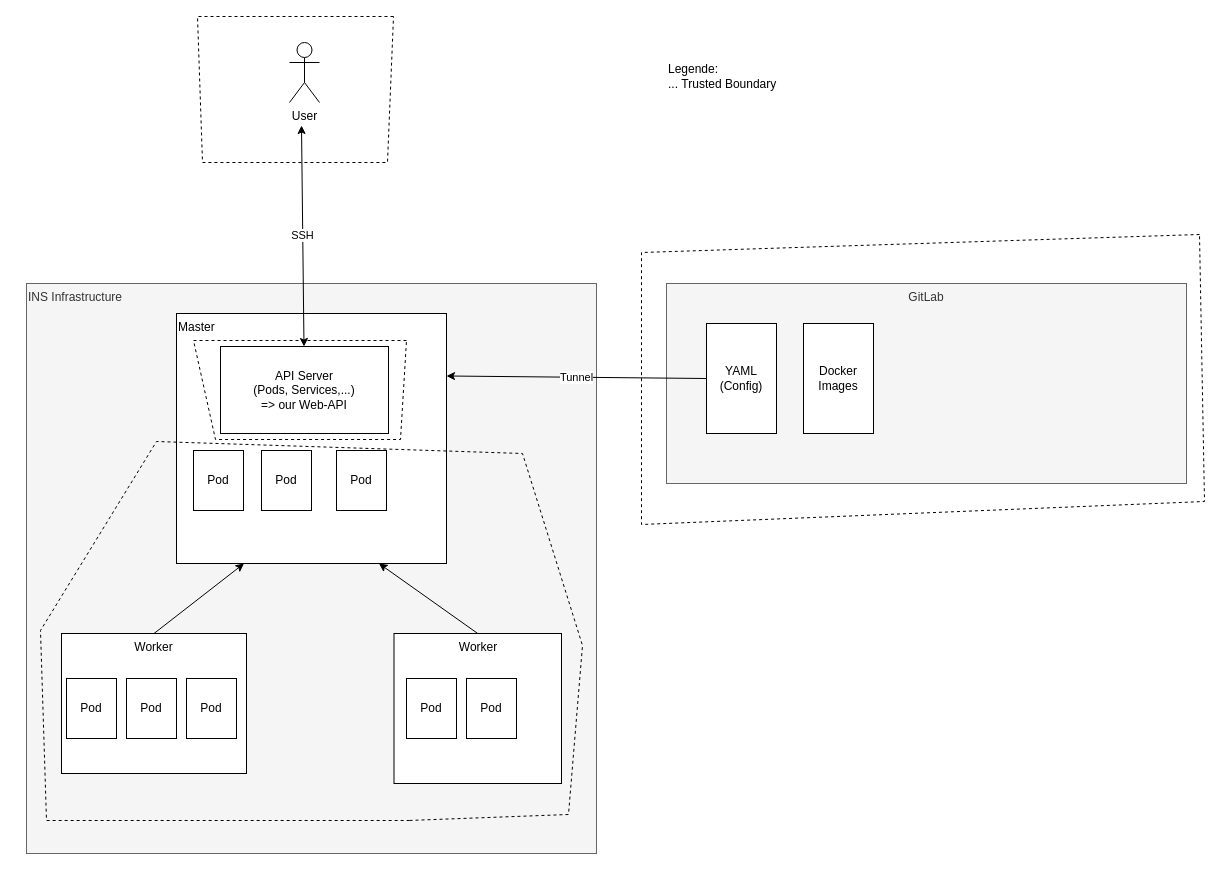
\includegraphics[height=12cm]{resources/architecture_threat_model.png}
\end{figure}


\newpage
\section{Threat Identification}
The following table includes all threats that we found in our architecture and are categorized in the STRIDE model categories.
\begin{longtable}[h!]{p{2.1cm} p{1.8cm} p{3cm} p{2cm} p{3.5cm}}
    \caption{\label{tab:threats-classification}Classification of identified threats}
    \endfirsthead
    \textbf{Component} & \textbf{Category} & \textbf{Threats} & \textbf{Risk} & \textbf{Mitigation} \\
    \endhead
    \hline
    User                & D, E & Worm & Low & \\
                        & & Residual risk & Low & \\
    \hline
    User \(\leftrightarrow\) Master   
                        & T & Redirects Data Flow & Low & use certificate on web server \\ 
                        & I & Eavesdropping & Medium & Data Encryption \\
                        & I & SQL Injection & Medium & Input validation \\
                        & D & Website Defacement & Low & ACL and Filtering \\
                        & D & Botnet Attack & High & CDN and redundant system \\
                        & & & & Patch Services \\
    \hline
    API server          & S & Session Hijacking & Medium & Instal SSL certificate \\
                        & T & SQL Injection & High & Input validation \\
                        & T & XSS & Medium & Input validation, alert system, santization \\
                        & R & Audit Log Deletion & Low & Backup audit log \\
                        & R & Insecure Backup & Low & implement digital signature and encryption \\
                        & I & Verbose Exception & Medium & Correct exception handling, no critical information disclosure \\
                        & D & Website Defacement & Low & ACL and Filtering \\
                        & D & Botnet Attack & High & CPU limitation, CDN and redundant system \\
                        & & Service vulnerability (later) & & \\
    \hline
    K8s Cluster             
                        & S & IP Redirection & Low & use certificate \\
                        & D & Hardware failure & Low & Keep backups of K8s configuration files \\
                        & D & Absorb CPU & Medium & logging and alert system \\
    \hline
    GitLab \(\leftrightarrow\) Master 
                        & T & Change packet content & High & digital signature \\
                        & I & Evesdropping & High & Data Encryption \\
                        & D & Tunnel is unresponsive for CI/CD & Low & Manual deployment of source code on K8s cluster \\
    \hline
    GitLab
                        & T & Malicious source code injected through automated GitLab Runner & Low & \\
    \hline
\end{longtable}


\section{Model Assumptions and Explanations}

\subsection{User}
\begin{itemize}
    \item Assumption: The user have read-only access to the web application because he just need to look at the cluster metrics.
    \item In a next step when the user need to change some data the login will be required and then the threat model needs to be updated to the authentication.
\end{itemize}


\subsection{Interface: User \(\leftrightarrow\) Kubernetes Master}
\begin{itemize}
    \item Assumption: the web app is only accessible from within INS.
    \item SQL Injection between Web App and database: mainly information disclosure, potentially Tampering to misrepresent the state of the nodes which are under a denial of service attack. This could pretend that the nodes are up and healthy, while the cluster is actually going down. However, the likelihood of this type of attack is rather low as it is questionable what the benefits are for an attacker. Unless there is a critical application running that may be the target.
    \item SSH connection between a user and K8s cluster: keep ssh service up to date, especially any TLS implementations to ensure authenticity and integrity.
    \item Potential extension: external web app / domain reqired \(\rightarrow\) requires user authentication \(\rightarrow\) update Threat model.
\end{itemize}

\subsection{API Server on Master}
\begin{itemize}
    \item A Master under DoS attack would prevent the API and the Server from running
        \begin{itemize}
            \item This is a dependency on the Master
            \item Mitigation: CPU limitation and alert to users
        \end{itemize}
    \item Potential extension of the threat model: if Web App is externally accessible user authentication is required to ensure only authorised users can access the monitoring and potentially the cluster data
\end{itemize}

\subsection{Cluster}
\begin{itemize}
    \item In-Cluster communication: how does the Master communicate with the Workers and the various Nodes?
    \item Potential extension of the threat model: depending on the protocol used the model has to take threats targeting this communication into account
\end{itemize}

\subsection{Interface Master \(\leftrightarrow\) GitLab}
\begin{itemize}
    \item Tunnel between the Master / Cluster and the GitLab pipeline is assumed to be low risk due to the default secure implementation nature of a tunnel. Of course, the same security issues for any component using TLS apply here as well.
\end{itemize}



\part{Project Documentation}
% Note: The project proposal needs to be included in the following way (i.e. using `\input` and not `\include`, and with the `\chapter` declaration outside the input{}-tag), since the proposal can also be generated as a stand-alone document.
\chapter{Initial Project Proposal}


\paragraph{Project name:} KubeWatch

\subsubsection*{Team Members}

\begin{compactenum}
    \item Petra Heeb (\href{mailto:petra.heeb@ost.ch}{petra.heeb@ost.ch})
    \item Benjamin Platter (\href{mailto:benjamin.plattner@ost.ch}{benjamin.plattner@ost.ch})
    \item Olivier Lischer (\href{mailto:olivier.lischer@ost.ch}{olivier.lischer@ost.ch})
    \item Jan Untersander (\href{mailto:jan.untersander@ost.ch}{jan.untersander@ost.ch})
    \item Pascal Lehmann (\href{mailto:pascal.lehmann@ost.ch}{pascal.lehmann@ost.ch})
\end{compactenum}

\subsubsection*{Availabilities}

% Table generated using https://www.tablesgenerator.com

\begin{flushleft}
    \begin{tabular}{|c|c|c|c|c|c|}
        \hline
        Time slot   & Mon & Tue & Wed & Thu & Fri \\ \hline
        08h00-09h00 & XR  & -  & -  & -  & -  \\ \hline
        09h00-10h00 & XR  & -  & -  & -  & -  \\ \hline
        10h00-11h00 & -  & -  & -  & (XO)  & -  \\ \hline
        11h00-12h00 & -  & -  & -  & (XO)  & -  \\ \hline
        \rowcolor[HTML]{EFEFEF}
        12h00-13h00 & XR  & XR  & XR  & XO  & XO  \\ \hline
        13h00-14h00 & -  & -  & -  & -  & -  \\ \hline
        14h00-15h00 & -  & -  & -  & -  & -  \\ \hline
        15h00-16h00 & -  & -  & -  & (XO)  & (XO)  \\ \hline
        16h00-17h00 & -  & -  & -  & (XO)  & (XO)  \\ \hline
        \rowcolor[HTML]{EFEFEF}
        17h00-18h00 & -  & -  & -  & XO  & XO  \\ \hline
        \rowcolor[HTML]{EFEFEF}
        18h00-19h00 & -  & -  & -  & XO  & XO  \\ \hline
    \end{tabular}

\end{flushleft}


\instructions{

    \noindent Please mark ALL time slots during which every team member can attend review meetings.

    \begin{flushleft}
        \begin{tabular}{|c|l|}
            \hline
            XO   & Slot available online                               \\ \hline
            XR   & Slot available in Rapperswil                        \\ \hline
            (XO) & Slot available online, but not optimal              \\ \hline
            (XR) & Slot available in Rapperswil, but not optimal       \\ \hline
            -    & Slot not available                                  \\ \hline
        \end{tabular}
    \end{flushleft}

    Having a slot available on campus automatically implies that this slot is also available online. The more slots that are available, the more likely it is that you will get an optimal slot and coach assignment. You are required to have a minimum of 5 slots available during regular working hours (08h-12h, 13h-17h) to be eligible to form a team.
}


\subsubsection*{Project Idea}

\instructions{ \noindent
    KubeWatch is a monitoring application for Kubernetes (K8S), intended for technical users.
    It keeps track of multiple K8S nodes, records performance data over time and generates visualizations from the aggregated data.
    It can detect when a node goes down, which triggers a notification to the person in charge.
    We chose this topic because it combines multiple technical aspects, so that each team member can get something out of it.
}

\noindent Ideas for extending the project scope:
\begin{itemize}
    \item Notifications through multiple channels like Email, SMS, IM.
    \item Running an analysis on the aggregated data to detect anomalies like a DDOS attack.
    \item Visualizing the K8S pods and nodes in a graph.
\end{itemize}

\subsubsection*{Proposed Realisation}

\instructions{ \noindent
    The K8S nodes are polled with the K8S API and the data ist stored in a database, since the K8S API doesn't deliver historical data.
    All interaction with the application happens through a web interface, which is backed by a Node.js server.
    We use Handlebars for templating and TypeScript for typesafe programming.
}\\
\\

\noindent We discussed our proposal briefly with Thomas Kälin and he approved of the direction we're going.

\chapter{Project Plan}

\instructions{
    Describe the project plan as covered in the SEP2 module. A project plan typically consists of the following topics:
    
    \begin{itemize}
        \item Processes, meetings and roles
        \item Phases, iterations and milestones
        \item A \textbf{rough} list of things to be done (work items)
        \item Risk management
        \item Planning Tools (issue tracker, time tracker, ...)
    \end{itemize}
    
    You should \textbf{\underline{not}} describe your \textbf{technical solution} in this chapter. It is all about organizing your project.
}
\chapter{Time Tracking Report}

\instructions{
    \section{How we track time}
    We record and plan all our tasks with individual issues on Gitlab.
    For every task we estimate how much time it's going to take and every team member reports his time spent on that task.
    The estimated and spent times are tracked with an accuracy of 15min.

    \section{Time tracking statistics}
    8 hours count as 1 day in this context.

    \subsection{Milestone 1: Project Plan}
    \begin{itemize}
        \item total estimate: 6d 2h 45m
        \item total spent: 5d 4h 45m
        \item The detailed report can be found \href{https://gitlab.ost.ch/SEProj/2022-FS/g03-kubewatch/kubewatch/-/blob/main/Documentation/time-tracking/M1\%20Project\%20Plan\%20Time\%20Tracking\%20Report.md}{here}.
    \end{itemize}
    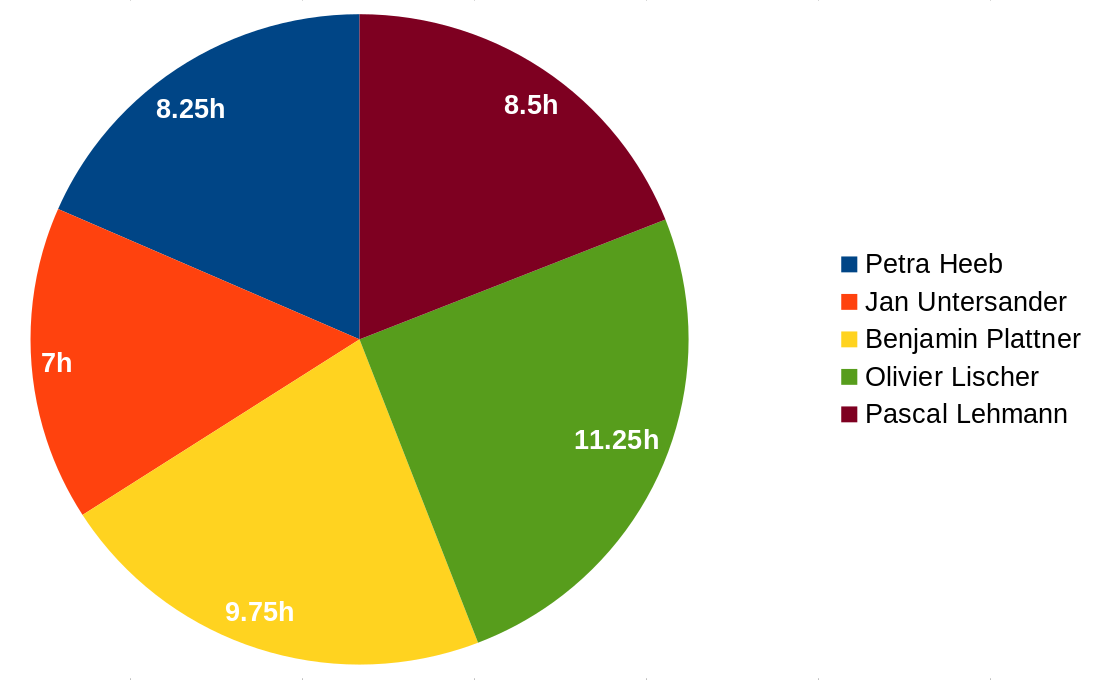
\includegraphics[width=10cm]{resources/m1_time_tracking_chart.png}

    \subsection{Milestone 2: Requirements}
    \begin{itemize}
        \item total estimate: 
        \item total spent: 
    \end{itemize}
}
% \chapter{Personal Reports}

\instructions{
    Before the final submission, \textbf{personally reflect} your work in this project:
    
    \begin{itemize}
        \item What things did go well?
        \item Which areas could we improve?
        \item What were your personal highlights?
    \end{itemize}
    
    The information gathered in this chapter will be \textbf{\underline{very}} useful for all your future projects.
}
\chapter{Meeting Minutes}

\instructions{
    Add your meeting minutes here. As usual, try to keep them short and concise. 
}
\chapter{Guidelines}
Project guidelines for Kubernetes resources as well as application coding guidelines.

\section{Kubernetes}
\begin{itemize}
    \item Configuration files written in yaml.
    \item Related objects are grouped in a single file if possible.
    \item Resource descriptions in annotations above resource definition.
    \item Use Deployment or StatefulSet to run workloads.
    \item Services are defined before corresponding workload.
    \item Filenames in snake\_case.
    \item Placeholder in angle brackets.
    \item Use label that define semantic attributes of the application or deployment. (Frontend,Backend,etc.)
\end{itemize}

\section{Web-API}
\begin{itemize}
    \item Use WebStorm's default linter to ensure conformity with the basic formatting rules, code smells, syntax, etc.
    \item Use WebStorm's default style guide for TypeScript
    \item Put CSS and JavaScript in separate files
    \item No JavaScript inline styles
    \item No HTML inline styles
    \item Variable names are in camelCase format
    \item All-caps for constant variables
    \item Boolean values start with is..
    \item Arrays have plural names
    \item Function names are verbs written in camelCase format
    \item Functions are short, handle one task, have as few arguments as possible, have a descriptive name, and do nothing else than what is implied
    \item Understandable, easily maintainable code that can be extended in a simple manner with straight forward troubleshooting is important
    \item Use NPM (Node Package Manager) for packages wherever possible
\end{itemize}
\chapter{Interface K8s Cluster and GitLab-OST}

\section{Overview}
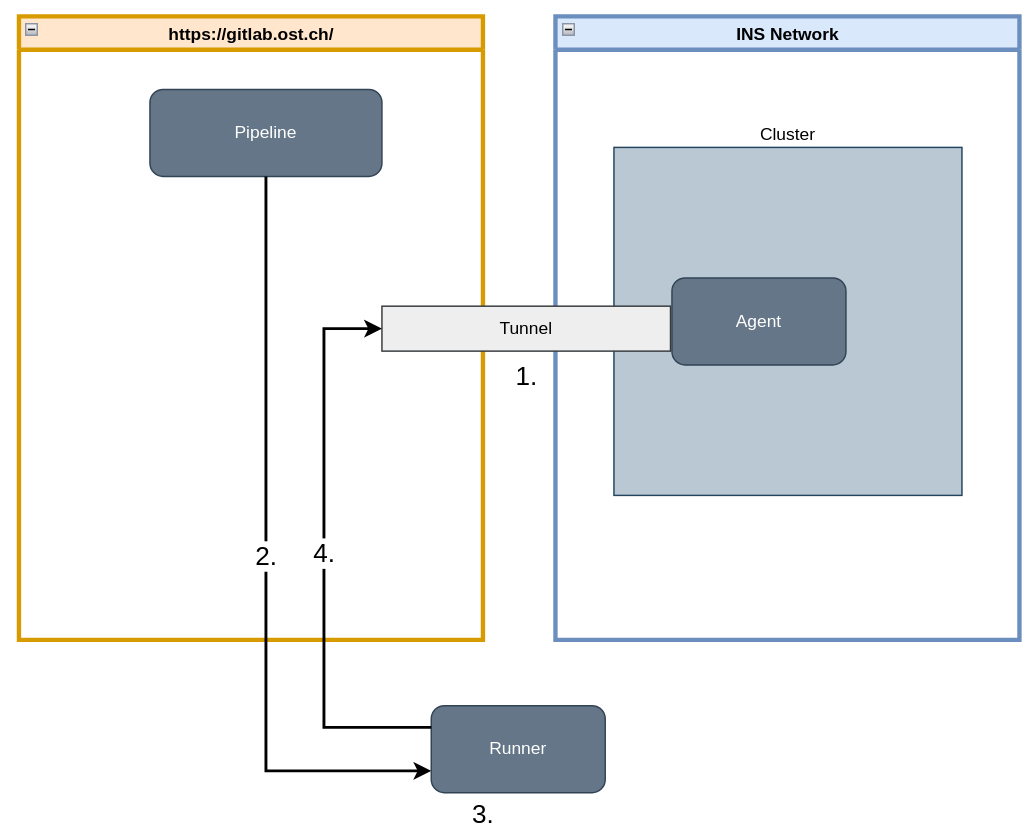
\includegraphics[height=12cm]{resources/k8s_including_in_gitlab-ost.png}
\begin{enumerate}
    \item The \textit{Agent} creates a \textit{Tunnel} from the INS network to the gitlab.ost.ch network.
    \item The \textit{Pipeline} triggers the \textit{Runner} to run the cluster commands.
    \item The \textit{Runner} starts the docker.
    \item The \textit{Runner} gets access to the \textit{tunnel endpoint} via the gitlab.ost.ch network and runs the cluster commands now at the cluster.
\end{enumerate}

\noindent The figure above shows how the Kubernetes cluster and GitLab are combined. GitLab and the cluster are in two different networks,  GitLab is placed in the OST network and the Kubernetes cluster is deployed in the INS network.

Only the \textit{Agent} inside the INS network can create the \textit{Tunnel} to the gitlab.ost.ch network. Nobody from the gitlab.ost.ch network can deploy the \textit{Tunnel} by themself.

The \textit{Runner} is independent of the location, so it does not depend on the network where you place the \textit{Runner}.

\section{Installation Agent in GitLab}
\begin{enumerate}
    \item Add the Kubernetes cluster in the GitLab project, it's important to add this configuration file at the correct path: `.gitlab/agents/ins-cluster-agent/ins-epj.yaml`
    \item Got to the \textbf{Infrastructure -> Kubernetes cluster} tab and install there a new agent (choose the ins-cluster-agent in the drop down menu)
    \item Safe the token! (Our Token: r8J8f3ve-DsU-v8cmrRSZx\_-atYyJqVCyePyk7zVCvSADy5-qg)
    \item Run the docker installation command from the popup window in you CLI (you need first to install docker locally)
    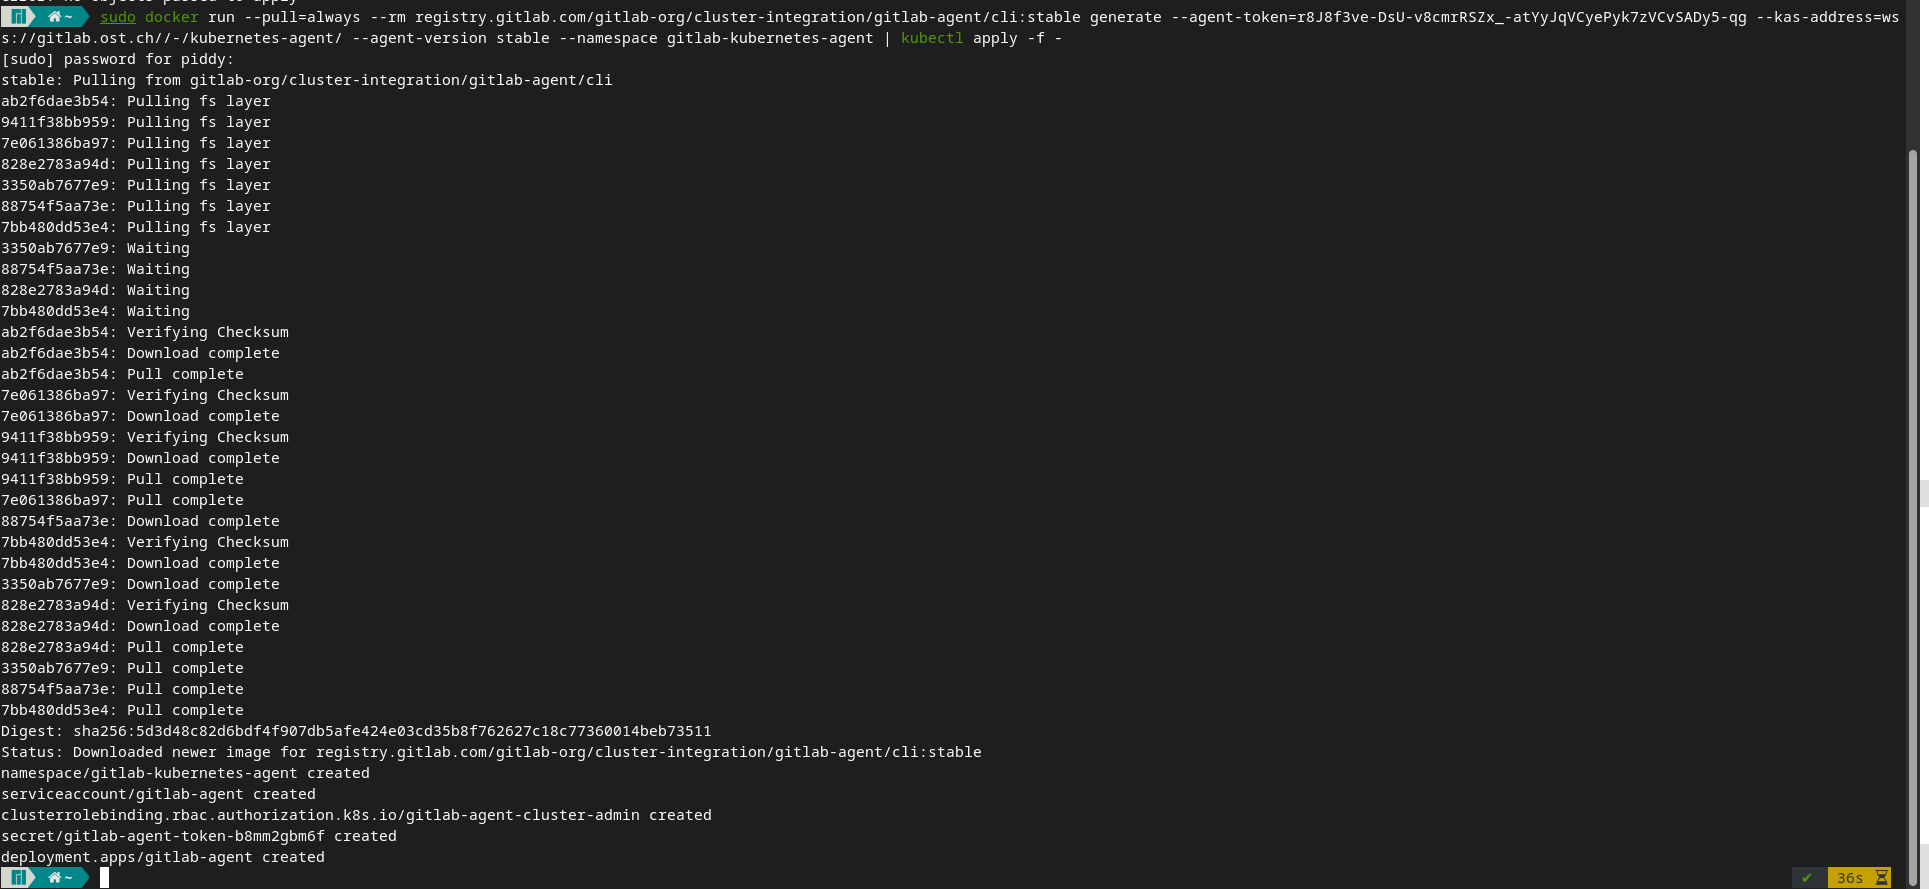
\includegraphics[height=5cm]{resources/agent-installation.png}
    \item Check if the connection in the GitLab is working
    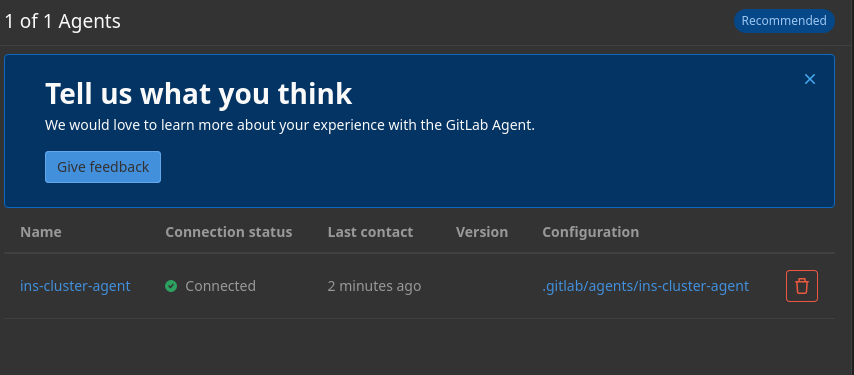
\includegraphics[height=5cm]{resources/ins-cluster-agent-connection.png}
    \item Check if the Cluster is running with the command kubectl config view (the output should be your agent configuration file)
    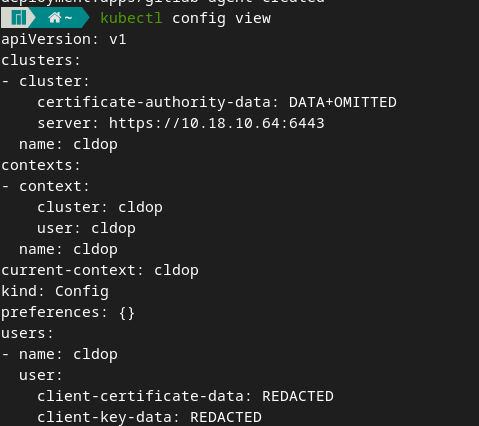
\includegraphics[height=5cm]{resources/ins-cluster-agent-accessing-cluster-test.png}
    \item update you .gitlab-ci.yml file to run kubectl commands
    \item update the agent configuration file for authorize the agent to access the project
\end{enumerate}
\chapter{Kubernetes Guide}

In this chapter we give a little kubernetes guide for the local installation and list the tools we need. All team members need to install the following tools/services.

\section{Installation}
\subsection{docker}
\href{https://docs.docker.com/get-docker/}{Docker Documentation}

\subsection{kubectl}
\href{https://kubernetes.io/docs/tasks/tools/#kubectl}{Kubernetes Documentation}

\subsection{minikube}
\href{https://minikube.sigs.k8s.io/docs/start/}{Minikube Documentation}

\subsection{cloud code}
\href{https://plugins.jetbrains.com/plugin/8079-cloud-code/}{Cloud Code Documentation(Webstorm plugin
)}

\section{Commands}
-- wichtigste commands

\section{Cloud Code Implementation}
-- erklären

\addcontentsline{toc}{chapter}{Bibliography}
\bibliographystyle{alpha}
\bibliography{bibliography}

\end{document}
